\documentclass[a4, 12pt]{article}

\usepackage[margin = 2cm]{geometry}
\usepackage{graphicx}
\usepackage{caption}
\usepackage{subcaption}
\usepackage{float}
\usepackage{hyperref}
\setcounter{secnumdepth}{0}

\usepackage{amsmath}
\usepackage{amssymb}
\usepackage{siunitx}
\usepackage{tcolorbox}
\usepackage{xcolor}
\usepackage{listings}

\definecolor{dkgreen}{rgb}{0,0.6,0}
\definecolor{gray}{rgb}{0.5,0.5,0.5}
\definecolor{mauve}{rgb}{0.58,0,0.82}
\lstset{frame=tb,
  language=c++,
  aboveskip=3mm,
  belowskip=3mm,
  showstringspaces=false,
  columns=flexible,
  basicstyle={\small\ttfamily},
  numbers=none,
  numberstyle=\tiny\color{gray},
  keywordstyle=\color{blue},
  commentstyle=\color{dkgreen},
  stringstyle=\color{mauve},
  breaklines=true,
  breakatwhitespace=true,
  tabsize=3
}



\title{STILL A DRAFT}
\author{MNXB01 \\ Philip J. Fredholm \\Lee Chun Hin }



\begin{document}
\maketitle
\tableofcontents
\newpage

\section{Introduction}
In order to be able to draw conclusions about some physical phenomena, such as the climate of Earth, it is sometimes necessary to be able to process large amounts of data. In order to save a considerable amount of time doing so, it is often the case that such processing may be done with the help of a computer programming language. The purpose of the subject of this report has been to try to use the programming language C++ in order to to process data from the SMHI OpenData initiative and draw conclusion about climate and weather trends from this data. In particular, attempts have been made in order to analyse the data and find the distribution of coldest and hottest day of each year, the first day of summer as well as to analyse the temperature of a given day of the year (August 23rd) over many years.

\section{Theory}
In order to be able make the analysis of what day is the first day of summer, a definition of when summer starts must first be laid out. The definition chosen for this project was 5 consecutive days of an average temperature greater or equal than 10.0 \textdegree C. \newline
\indent In order to be able to read in the data to be analysed, a class called \texttt{readData} , in C++ code according to the C++17 standard, was created and used by placing a source file in a folder called \texttt{src} and a header file in a folder called \texttt{include} inside the folder called \texttt{PhilipCode} [1]. The class \texttt{readData} would take a file name for a file as the same folder as the final program and how many header lines of a text file with relevant (and properly formatted) data to read in. It would then have three getter-functions, one to get the first year of measurements, one to get the last year where the data had measurements, one to get the file name of the read in file and finally one to get the data that was read in. The read in data was stored in in a vector from the C++ standard library, which in turn contained one vector for each year that there had been measurements. Each vector for a year in turn contained twelve vectors, one for each year. Finally, each 'month-vector' contained 31 vectors, one for each possible day, within which (that is to say within the 'day-vectors') the average of the measured values for that day was stored. If no measurements were available for a given day, that 'day-vector' was left empty. \newline
\indent In order to actually find the warmest and coldest day of each year, as well as the start of summer, a file called \texttt{main.cpp} was placed in the folder \texttt{PhilipCode} and when compiled had access to the \texttt{dataReader} class by being compiled with a translation unit. This \texttt{main.cpp} file contained a function for finding either the hottest or coldest day of a given year by taking a pointer to a 'year-vector' of the type that was stored in the vector given by the getter function for the data of the \texttt{readData}-class. Similarly, there was also a function for finding the first day of summer, according to the definition presented earlier, by taking a pointer to a 'year-vector'. It should be noted that the way these functions operated was by creating a 'flattened' vector, which created a vector of as many elements as there were (nested) day vectors in the 'year-vector' given to the function as an argument. If a day had no measured values, it was still added to the 'flattened' vector and given a 'garbage' value, either extremely big or extremely small, as to not interfere with the logic used to find the desired day. It is important to note that since the 'year-vectors' month vectors always had 31 'day-vectors', the number of days in the flattened vector was always greater than 366, as even days which do not exist, such as a February 31st, were still added as a 'garbage' value. Finally, the \texttt{main.cpp} created output files storing the hottest and coldest days found of each year by the index of the hottest day in the flattened year vector. It also outputted a datafile with the index of the first day (in the flattened year vector) of the first day to meet the previously stated requirement for the start of summer. \newline \indent
In order to plot the results, three ROOT macros, called \texttt{hot.C}, \texttt{summer.C} and \texttt{summer.C}, and placed in the \texttt{PhilipCode} folder, were used. These macros read in the relevant data file created from the \texttt{main.cpp} file and created histograms with 366 bins from one to 366. It then added the number of counts from the read in processed data to the relevant bins. Note that for the macro \texttt{cold.C}, there was instead 400 bins between $-200$ and 199, and all counts for days with day number greater than 180 were given to the bin which had day number of 365 less than the relevant day. Note also that these 'days' give the day out of a 'year' where each of the twelve months have 31 days. The macros then also saved the histograms as graphs and printed the mean value of the day from the read in data and printed it to the standard output. Note that in [1] the macros, along with the processed data, have been moved to a folder called \texttt{rootmacros} in the folder \texttt{PhilipCode}.


\section{Method}
The \texttt{main.cpp} file was compiled using \texttt{g++} with an object file for the translation unit for the \texttt{readData}-class and the flags \texttt{-Wall}, \texttt{-Wextra} and \texttt{-Werror} and the version flag \texttt{-std=c++17}. The compilation was with the help of a program called \texttt{Make}. The outputted file was then ran, with the relevant data file to read from being placed in the same directory as the file which was ran, and data files containing the processed data were outputted. Following this, ROOT version 6.26/06 for Ubuntu 20 was ran on Ubuntu 20, running through Windows subsystem for Linux (WSL2). The macros \texttt{hot.C}, \texttt{cold.C} and \texttt{summer.C} were compiled with the \texttt{.L <filename>+}-syntax. The defined functions in these macros were then ran and the outputted values of the means were read off from the the standard output and the generated histograms were saved.



\section{Results}
The mean day as for being the coldest day of the year was found to be day $31.6812$, the mean day for being the coldest day of the year was found to be day $ 192.428$ and the mean day to be the start of summer was found to be day $139.051$. The respective histograms for coldest and hottest days, as well as for the first day of summer, may be seen in Figure 1, Figure 2 and Figure 3 respectively.


%Philip's Figures

\begin{figure}[H]
\centering
\begin{subfigure}{.5\textwidth}
  \centering
  \captionsetup{width = 0.9\linewidth}
  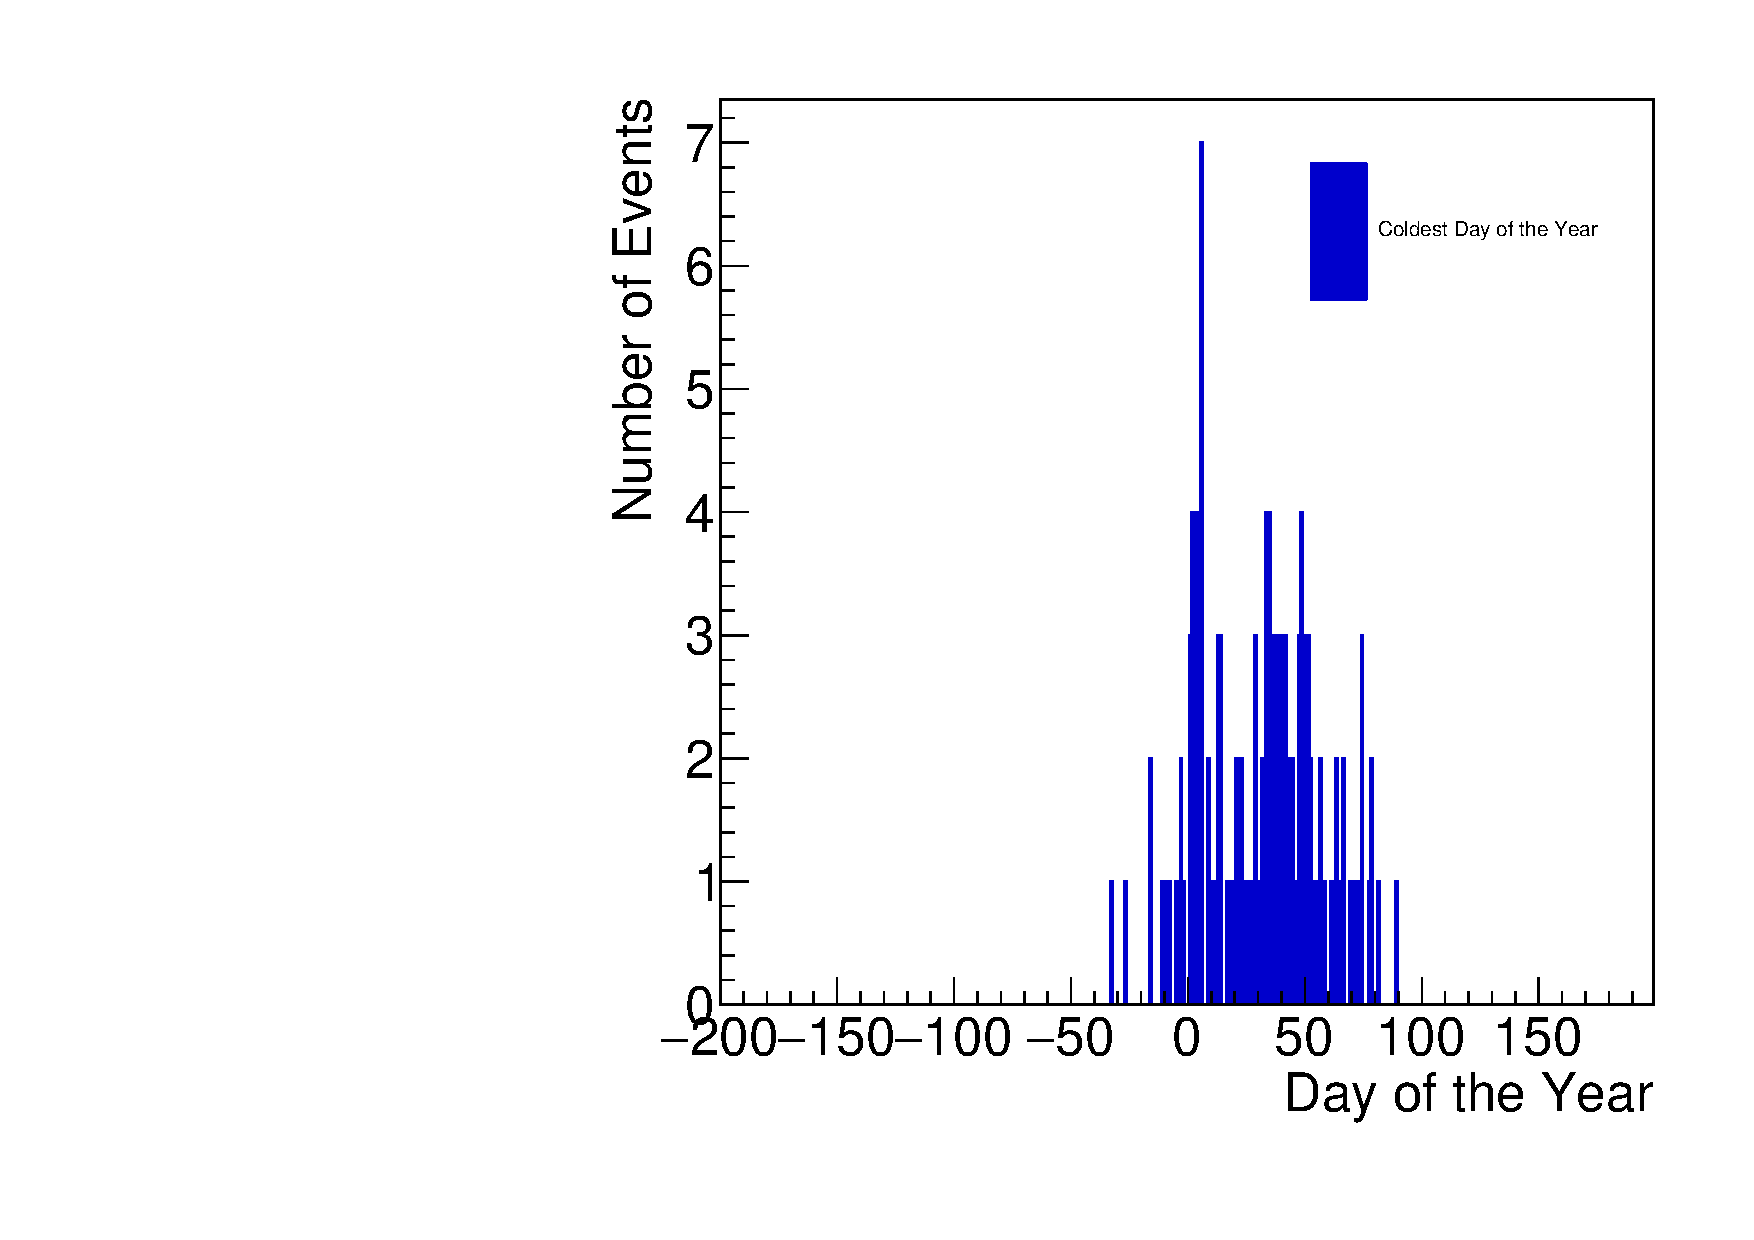
\includegraphics[width=0.9\linewidth]{philipCold.pdf}
   \caption*{Figure 1: Shows the number of occurrences of a specific day being the coldest day of that year in Borås. Negative days indicate that the day was in the end of the previous year and its value for the day was shifted back 365 days. Note that the 'days' given here is the day out of a year where each of the twelve months are taken to have 31 days.
   }
\end{subfigure}\hfill
\begin{subfigure}{.5\textwidth}
  \centering
  \captionsetup{width = 0.9\linewidth}
  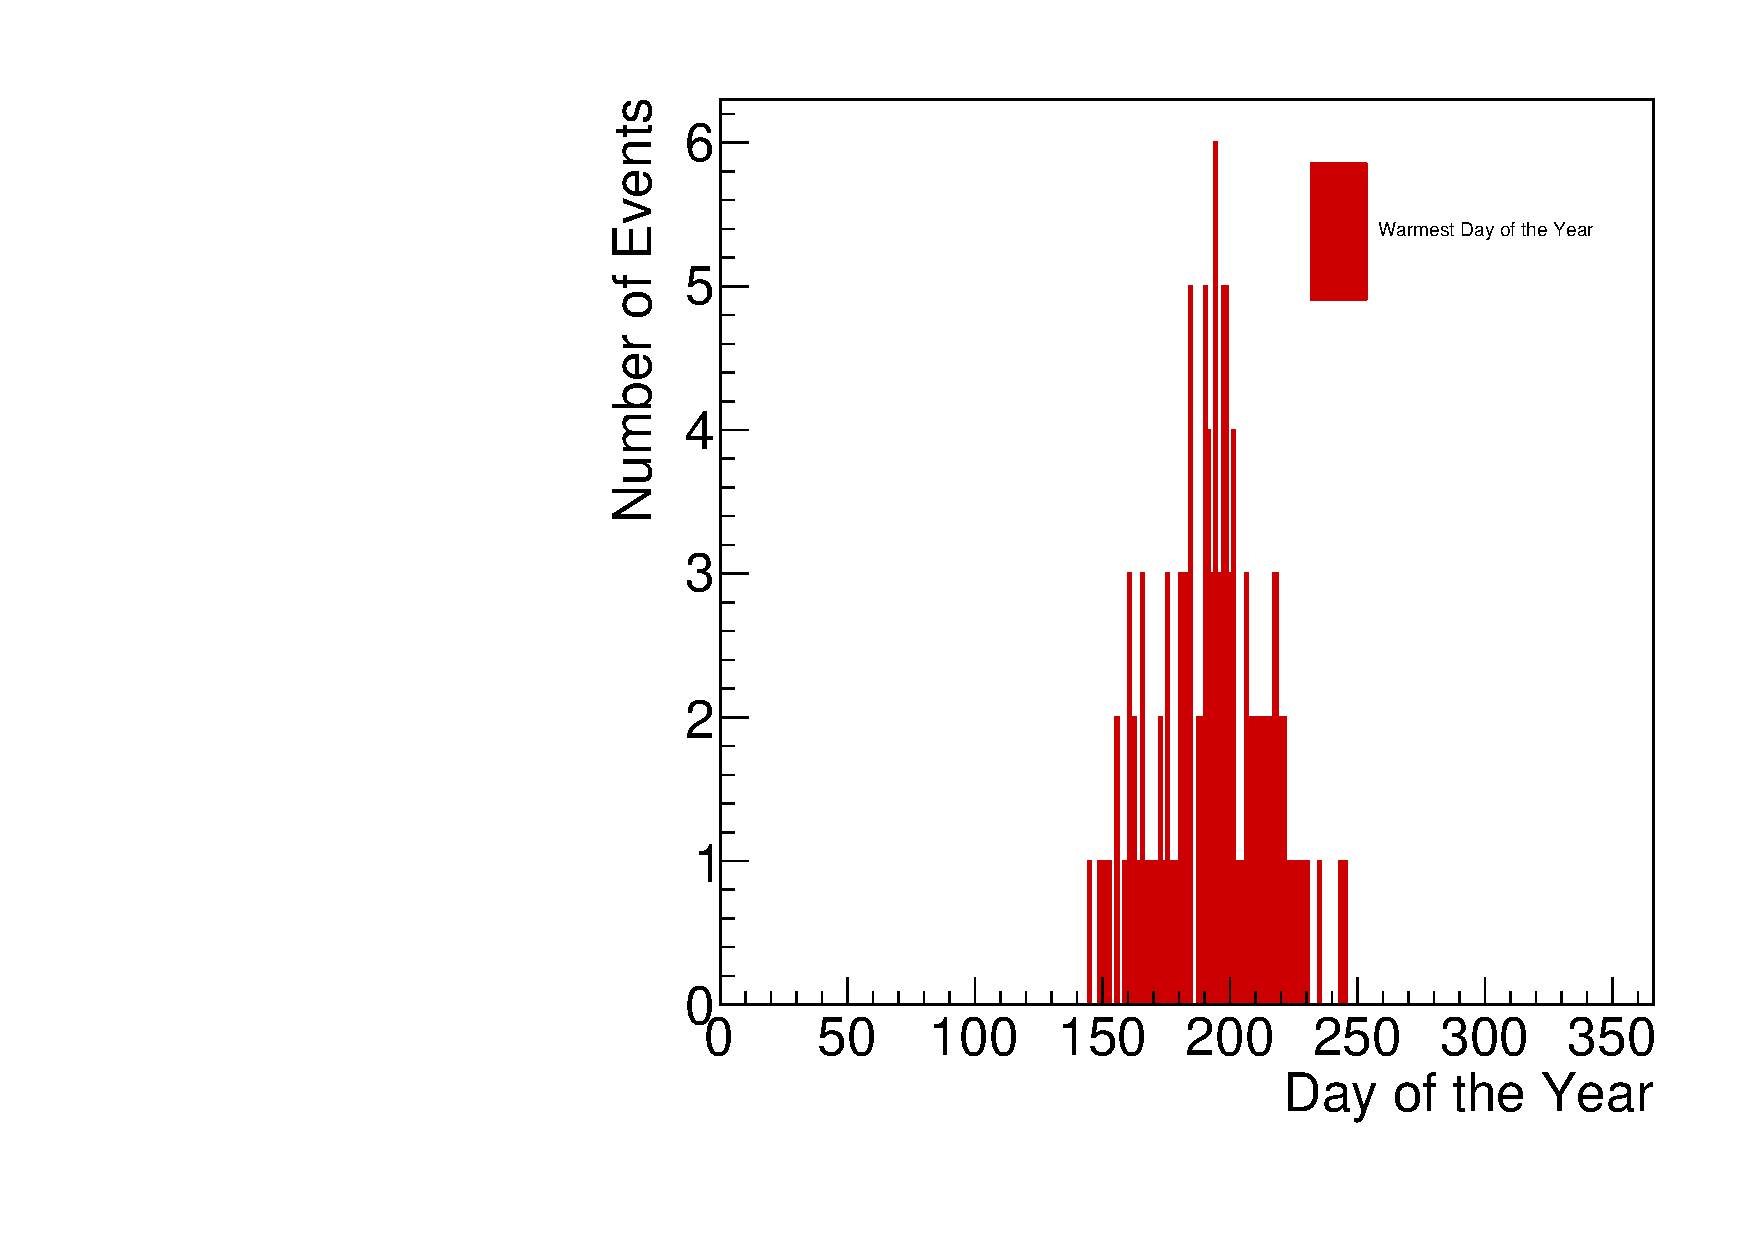
\includegraphics[width=0.9\linewidth]{philipHot.pdf}
  \caption*{Figure 2: Shows the number of occurrences of a specific day being the warmest day of that year in Borås. Note that the 'days' given here is the day out of a year where each of the twelve months are taken to have 31 days. \newline \newline \newline  \mbox{         }}
\end{subfigure}

\end{figure}



\begin{figure}[H]
\centering
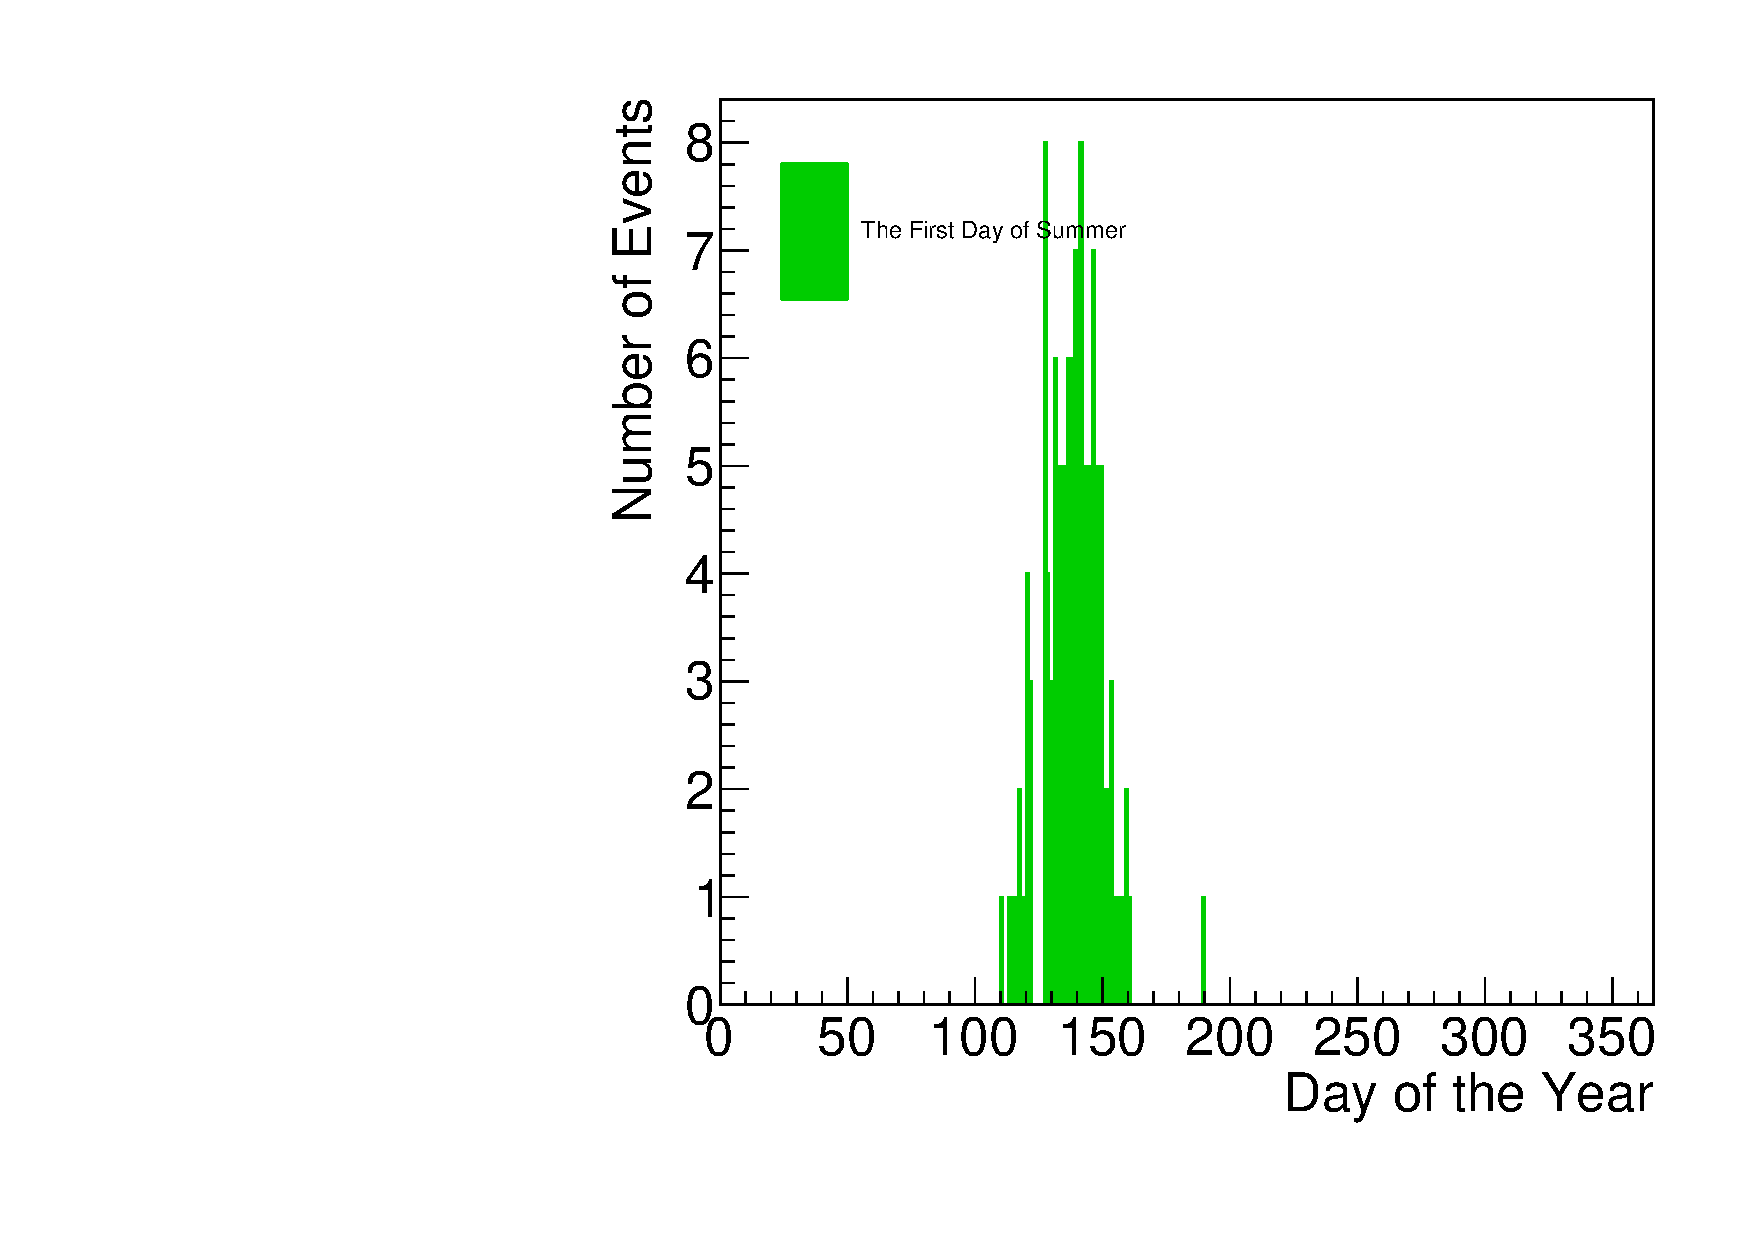
\includegraphics[scale=0.45]{philipSummer.pdf}
\caption*{Figure 3: Shows the number of occurrences of a specific day being the first day of summer that year in Borås. Note that the 'days' given here is the day out of a year where each of the twelve months are taken to have 31 days.}
\end{figure}
\newpage




%Chris's Figures


\begin{figure}[H]
\centering
\begin{subfigure}{.5\textwidth}
  \centering
  \captionsetup{width = 0.9\linewidth}
  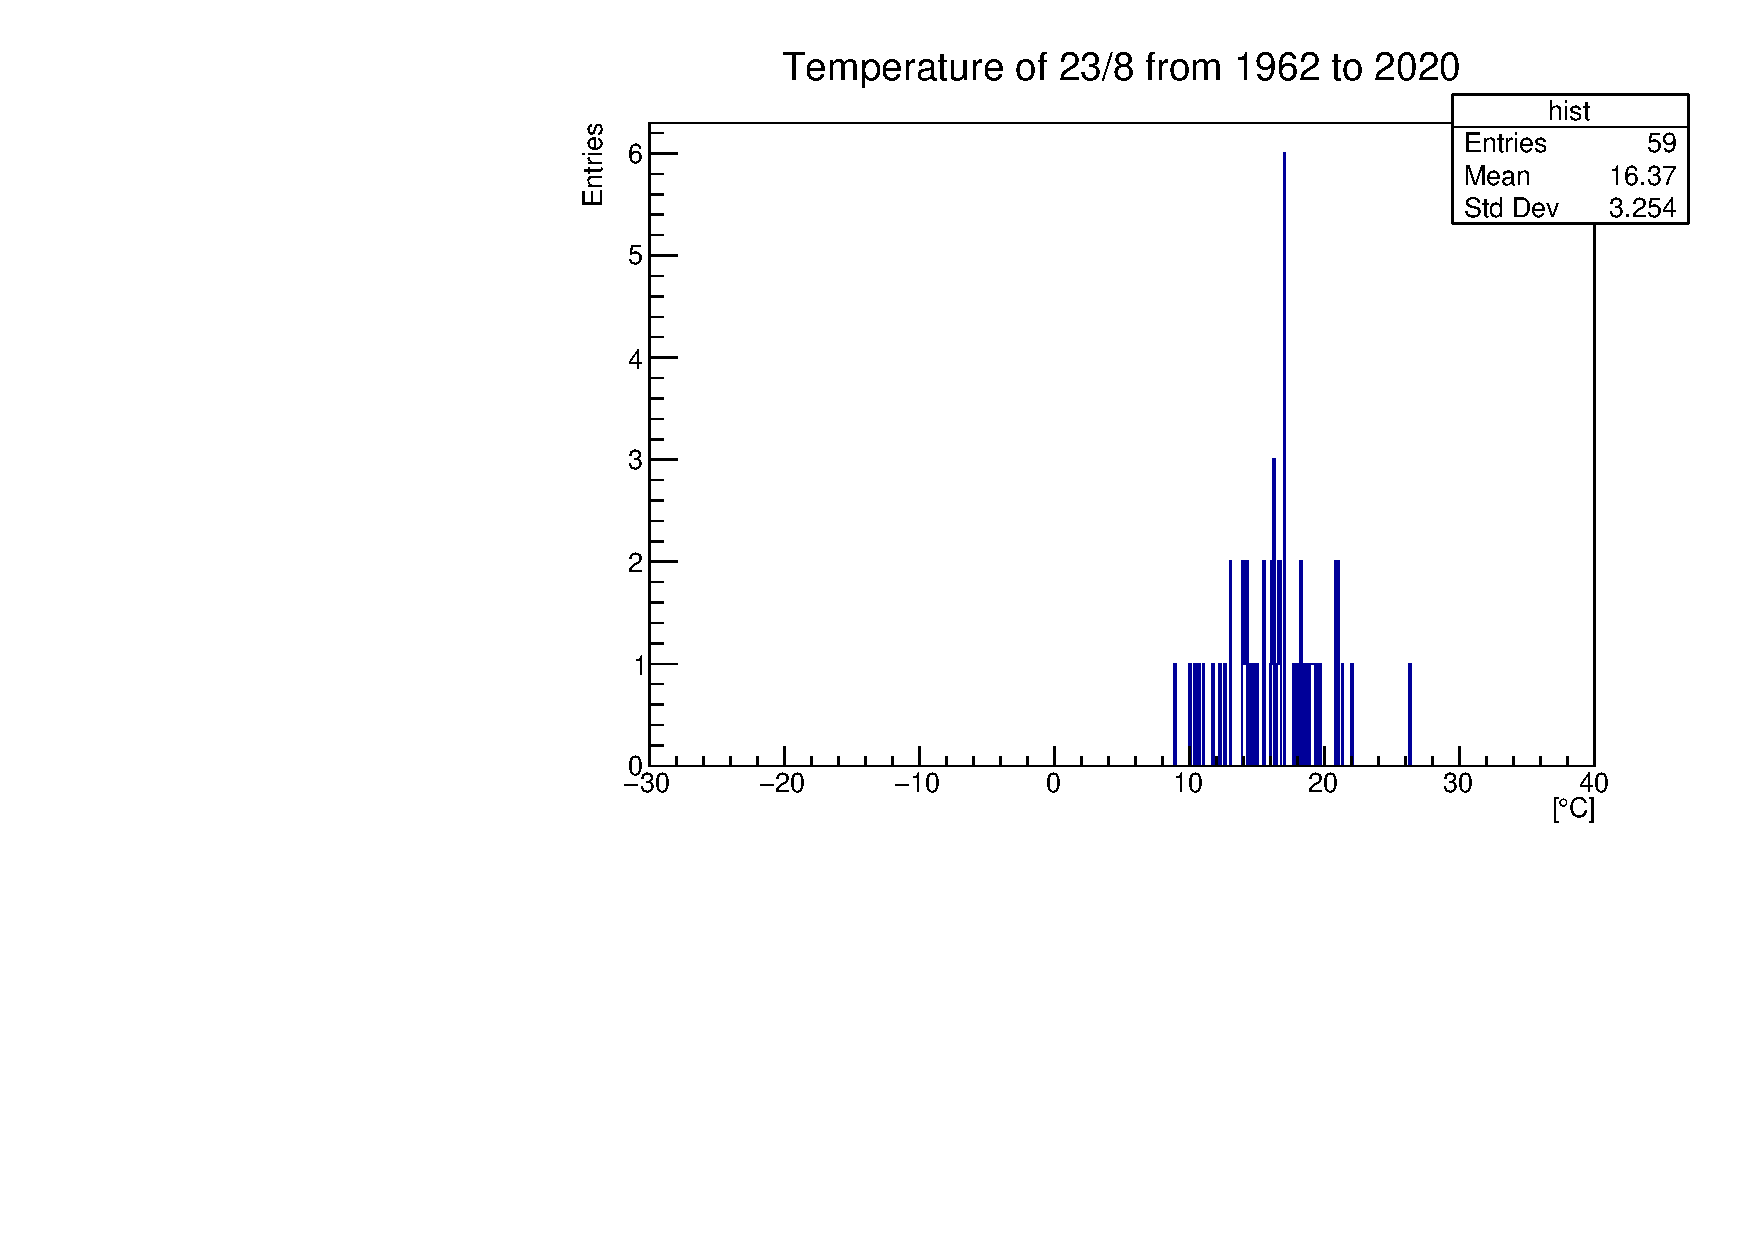
\includegraphics[width=0.9\linewidth]{chrisFig1.pdf}
   \caption*{}
\end{subfigure}\hfill
\begin{subfigure}{.5\textwidth}
  \centering
  \captionsetup{width = 0.9\linewidth}
  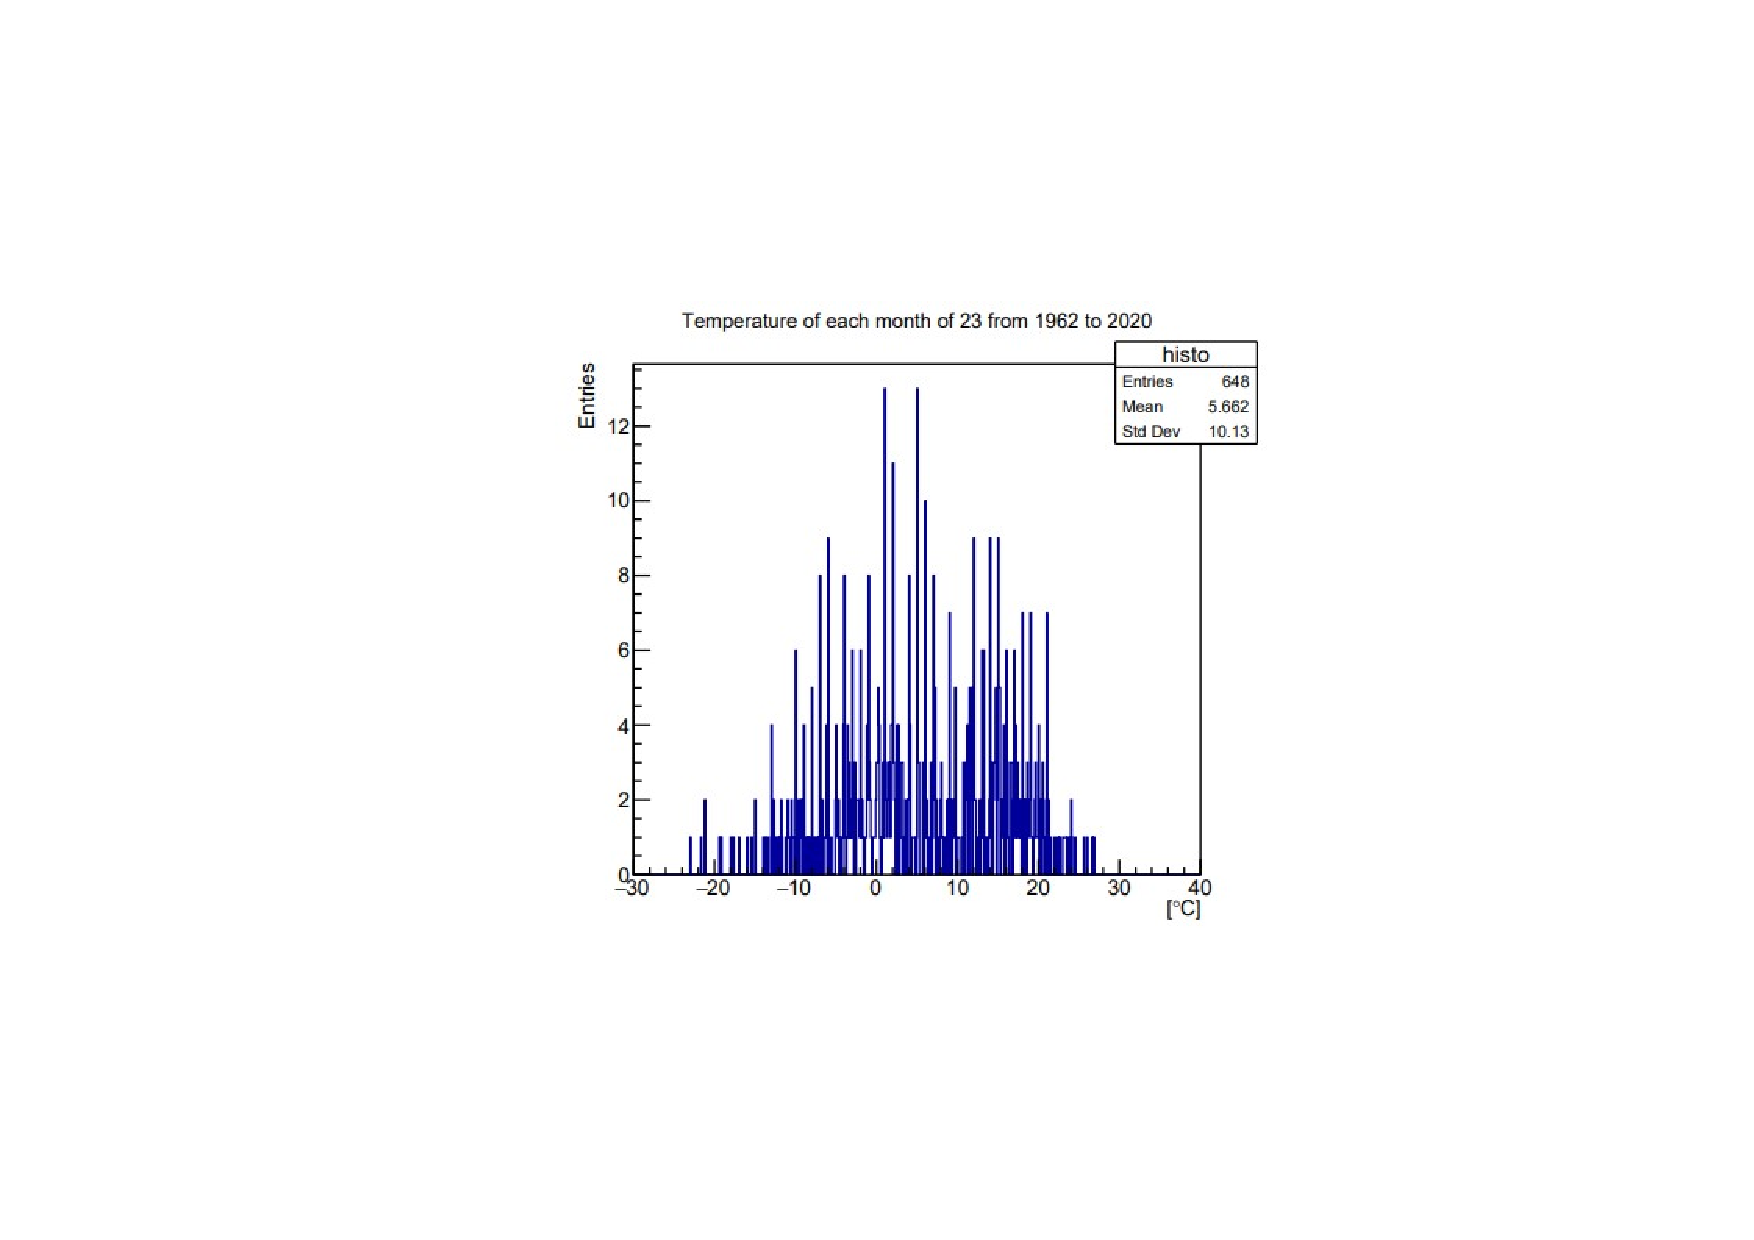
\includegraphics[width=1.5\linewidth]{chrisFig3.pdf}
  \caption*{}
\end{subfigure}

\end{figure}

\begin{figure}[H]
\centering
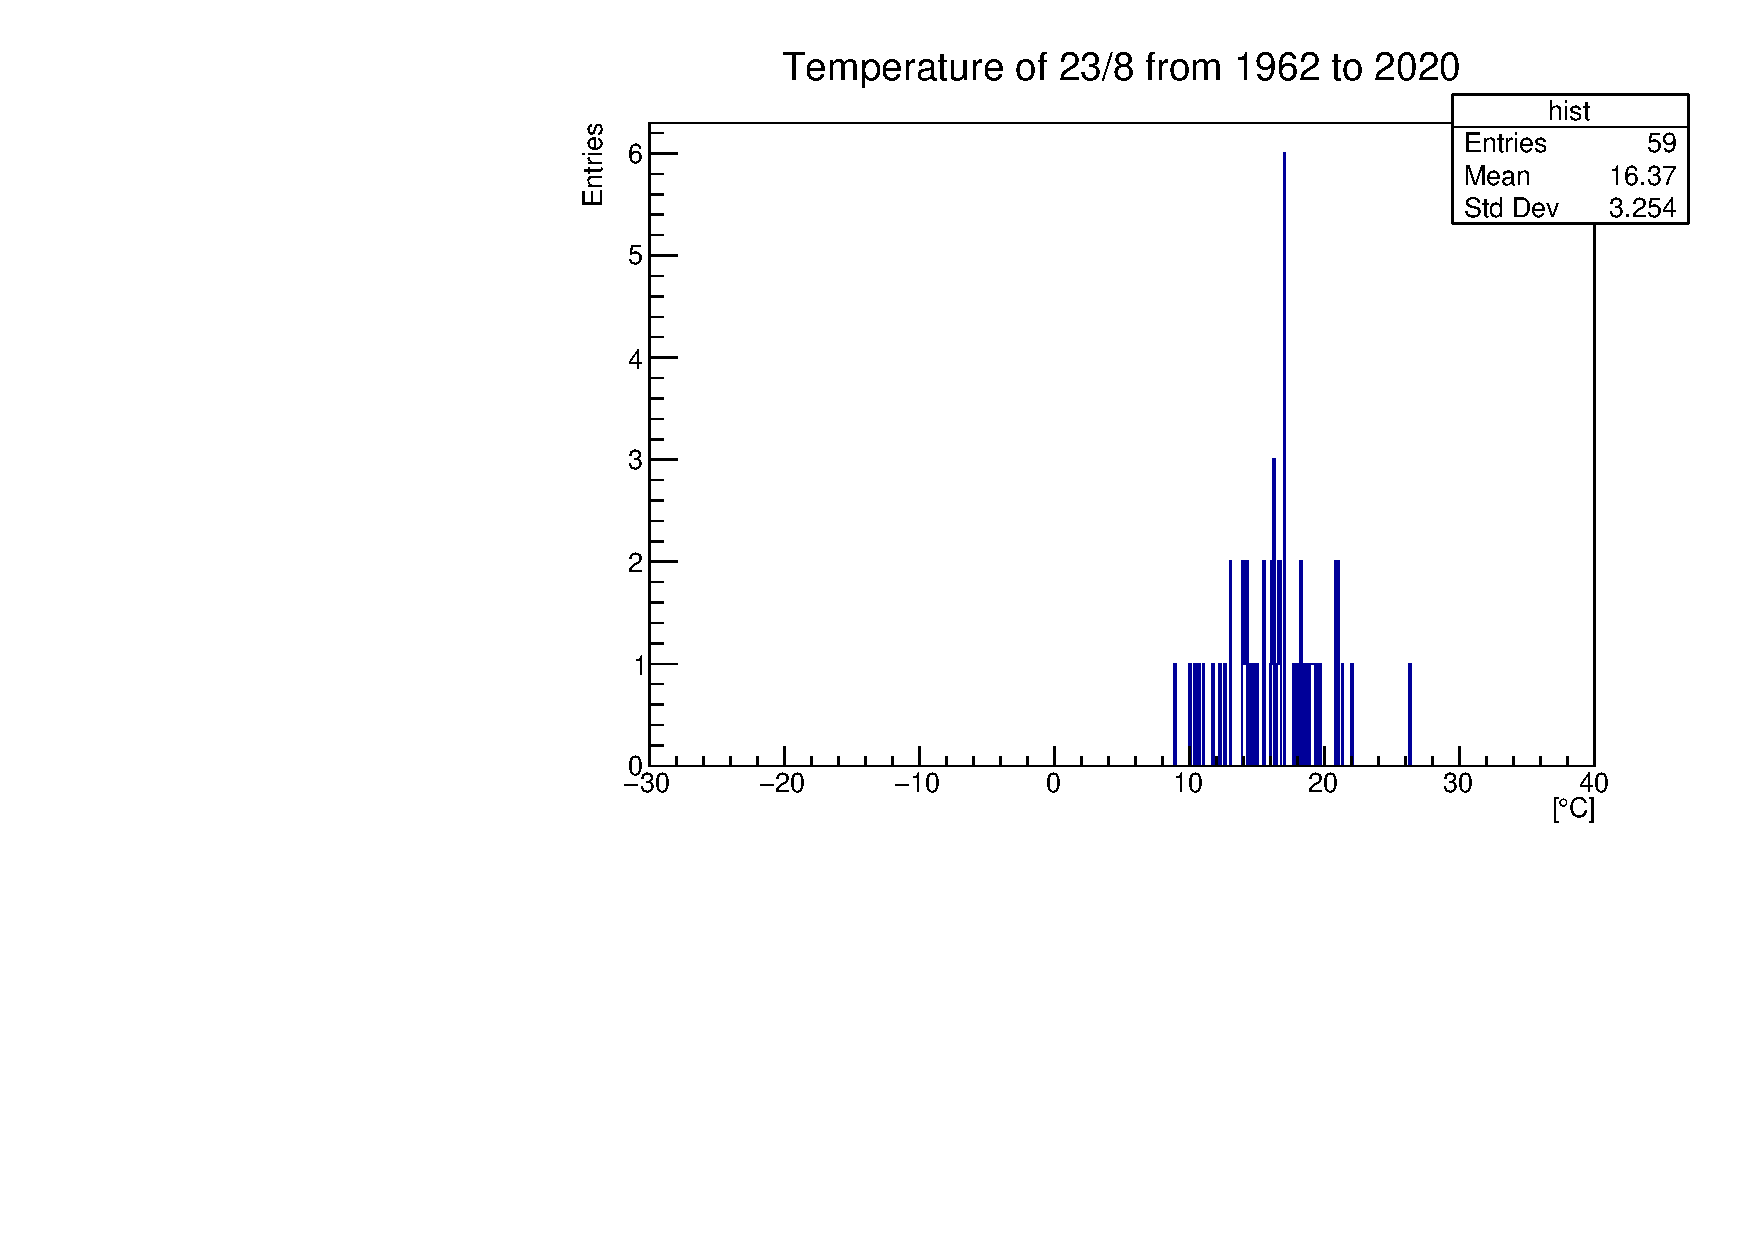
\includegraphics[scale=0.6]{chrisFig1.pdf}
\caption*{Figure 4: Temperature of Umeå Airport in 23/8 from 1962 to 2020.}
\end{figure}


\begin{figure}[H]
\centering
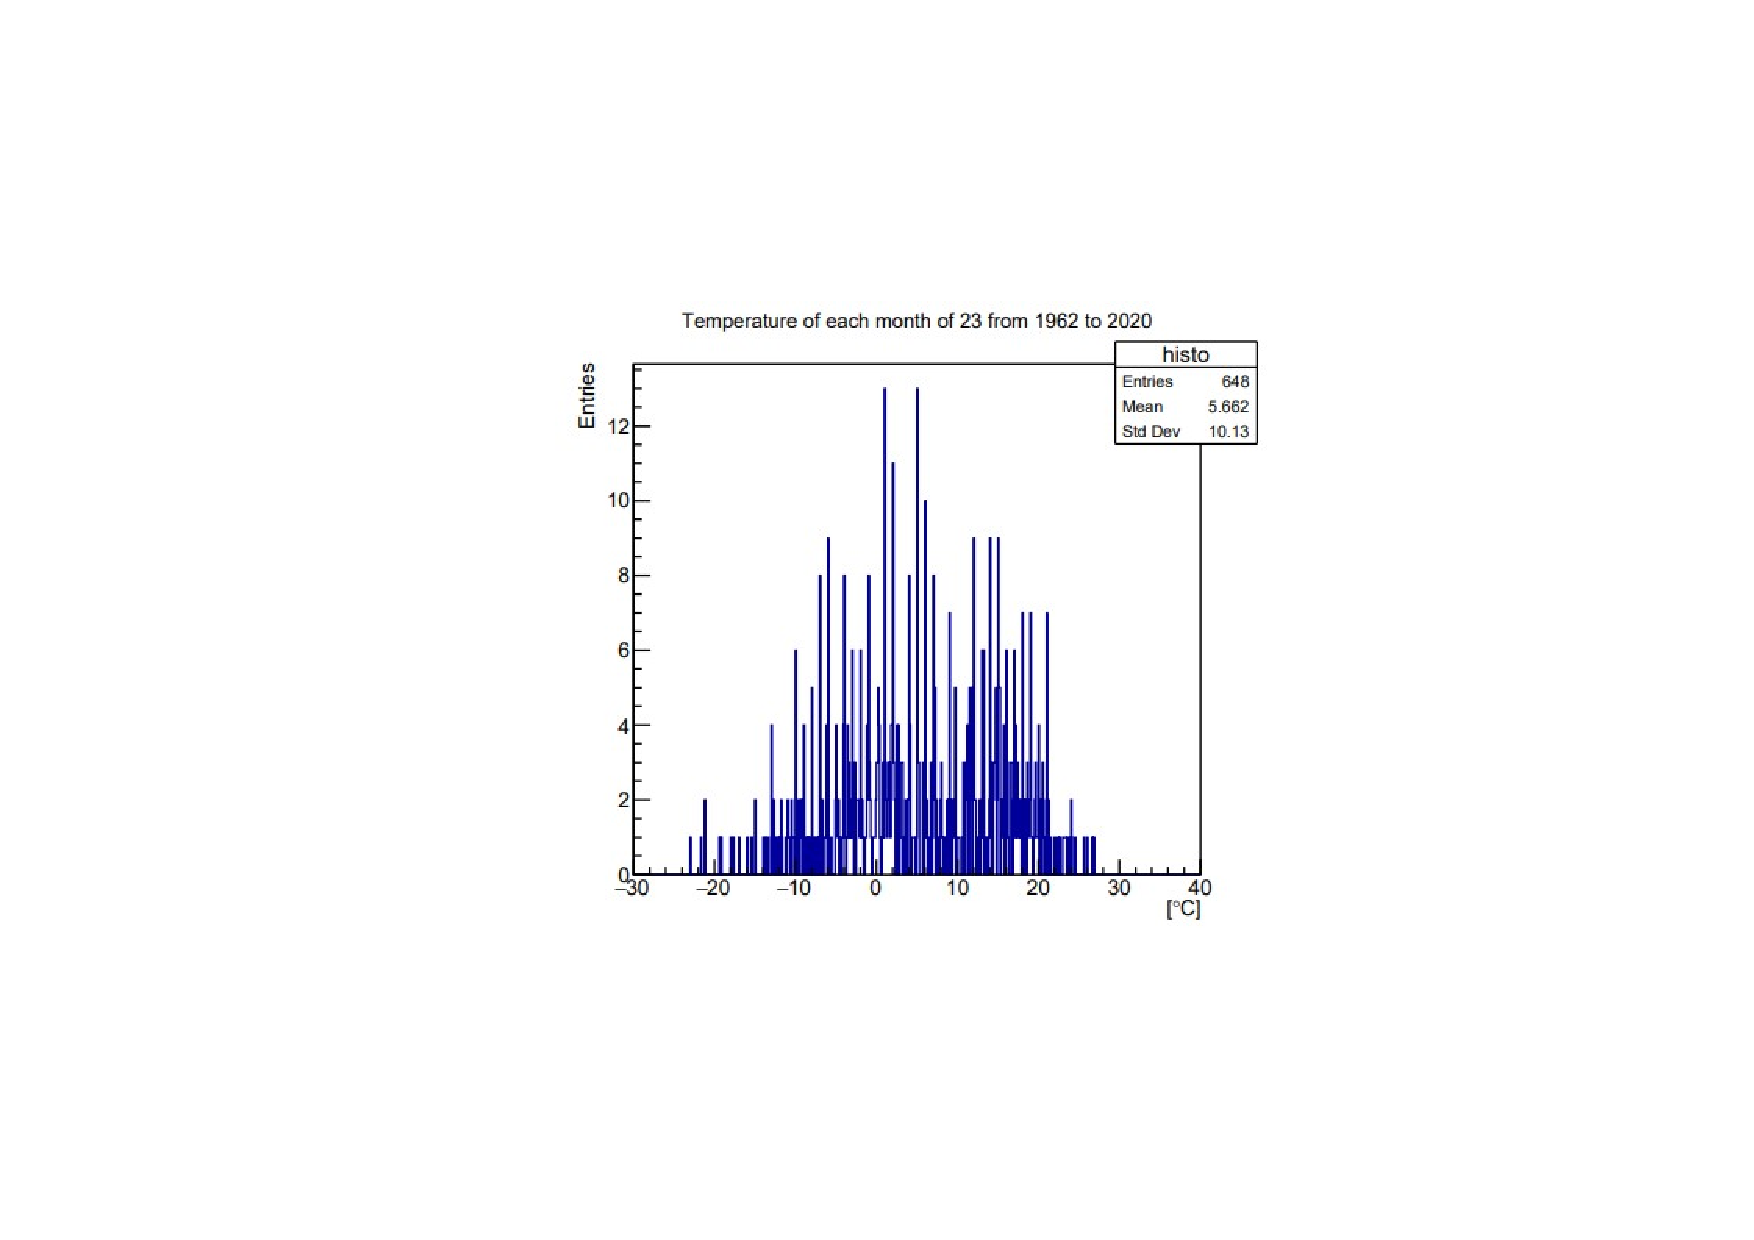
\includegraphics[scale=0.7]{chrisFig3.pdf}
\caption*{Figure 5: Temperature of Umeå Airport in each of the date of 23 since 1962 to 2020.}
\end{figure}




%Figure 1.1 shows the temperature for each month of 23/8 from 1962 to 2020.The mean temperature and the standard deviation is 16.37 and3.254 respectively.We can predict the probability of particular tmeperature by using the mathematical below:
%Z=(X-μ)/σ where Z=Standard score,,σ=standard deviation,μ=population mean
%For example if we want to predict what is the probability for the coming 23/8 to be in the temperature of 12°c.By applying the above equation,
%Z=(12-16.37)/3.254
%Z=-1.34
%By looking the table below(figure1.2), we can observe the probability of different value of standard score.

%In this case, the probabilty will be in0.09.

%Figure 1.2 show each of the date 23 in every month since 1962 to 2020. The mean and the standard deviation are 5.662 and 10.43 respectively.
%As discussed above, we can use the same formula to predcit the temperature of the coming date 23 for having specific temperature.

%Figure 1.1 having a lower standard deviation than figure 1.2, which means that the data in fig.1,1 are more less disperse and more closing to the mean, which lead to a more focusing graph.




\section{Discussion}
%In order to make the histogram, i have use of the excel and root. Firstly, I use the finding function in excel to locate the string or the data I need. However, it is in a string format, and i need to separate the temperature data from the string. Hence i make use of the data analysis function in excel. It can sepraate the string by detecting each of the symbol(such as ;,) in the string. As a result i can seprate the temperature data I need from the original excel file.After that I use Win Zip to transfer the revised data to Auora. For the coding part, I create a new canvas named as c1 and with the title of Temperature of Umeå FLyplats. SInce I want to show the two graphs in the same page and in parllel, so i make use of the function of Divide(2,1). After that I create a histogram named as hist with the x,y axis be [°c], and Entries respectively. And the pixels of the histogram is set to 700. Besdies, the range of x axis is from -30 to 40. Then, I try to input the data file which named as 8-23Temp.txt into the histogram by using the command ifstream infiles and infiles.open. After that i store the data in a variable named as tmp by using the command double.

\newpage
\section{References}
[1] The code in the folder "PhilipCode", available on a remote Git repository on GitHub at \href{https://github.com/fredholmP/MNXB01-FinalProject}{https://github.com/fredholmP/MNXB01-FinalProject} . \newline

\noindent [2] The code in the folders INSERT CHRIS'S FOLDERS LOCATION HERE available on a remote Git repository on GitHub at \href{https://github.com/fredholmP/MNXB01-FinalProject}{https://github.com/fredholmP/MNXB01-FinalProject} . \newline

\noindent [3] The data available from January 1st 1884 at 07.00 up until June 1st 2021 at 06.00 for the city Borås, provided by Lund Univeristy in association with the course MNXB01 during the autumn semester of 2022. At the time of writing, this data may be downloaded from the website \href{https://www.smhi.se/data/meteorologi/ladda-ner-meteorologiska-observationer}{https://www.smhi.se/data/meteorologi/ladda-ner-meteorologiska-observationer}  . \newline


\noindent [4] The data available from DAY TIME up until DAY TIME for the "Umeå Flygplats" measuring station, provided by Lund Univeristy in association with the course MNXB01 during the autumn semester of 2022. At the time of writing, this data may be downloaded from the website \href{https://www.smhi.se/data/meteorologi/ladda-ner-meteorologiska-observationer}{https://www.smhi.se/data/meteorologi/ladda-ner-meteorologiska-observationer} . 






\end{document}
